\documentclass[draftthesis,tocnosub,noragright,centerchapter,12pt]{uiucecethesis09}

% Use draftthesis for notes and date markings on every page.  Useful when you
%   have multiple copies floating around.
% Use offcenter for the extra .5 inch on the left side. Needed with fullpage and fancy.
% Use mixcasechap for compatibility with hyperref package, which does NOT like all caps default
% Use edeposit for the adviser/committee on the title page.
% Use tocnosub to suppress subsection and lower entries in the TOC.
% PhD candidates use "proquest" for the proquest abstract.

\makeatletter

\usepackage{setspace}
\usepackage{epsfig}  % for figures
\usepackage{graphicx}  % another package that works for figures
\usepackage{pgfplots}
\usepackage{subcaption}  % for subfigures
\usepackage{amsmath}  % for math spacing
\usepackage{amssymb}  % for math spacing
\usepackage{bm}
%\usepackage{url}  % Hyphenation of URLs.
\usepackage{lscape}  % Useful for wide tables or figures.
\usepackage[justification=raggedright]{caption}	% makes captions ragged right - thanks to Bryce Lobdell

% Uncomment the appropriate one of the following four lines:
\msthesis
%\phdthesis
%\otherdoctorate[abbrev]{Title of Degree}
%\othermasters[abbrev]{Title of Degree}

\title{Frequency Modulated Continuous Wave Radar Processing Fundamentals}
\author{Kirk Busche}
\department{Electrical and Computer Engineering}
\degreeyear{2019}

% Advisor name is required for
% - doctoral students for the ProQuest abstract
% - master's students who do not have a master's committee
\advisor{Minh Do}

% Uncomment the \committee command for
% - all doctoral students
% - master's students who have a master's committee
%\committee{Professor Firstname Lastname, Chair\\
%        Professor Firstname Lastname} % etc.

\begin{document}

%%%%%%%%%%%%%%%%%%%%%%%%%%%%%%%%%%%%%%%%%%%%%%%%%%%%%%%%%%%%%%%%%%%%%%%%%%%%%%%
% COPYRIGHT
%
%\copyrightpage
%\blankpage

%%%%%%%%%%%%%%%%%%%%%%%%%%%%%%%%%%%%%%%%%%%%%%%%%%%%%%%%%%%%%%%%%%%%%%%%%%%%%%%
% TITLE
%
\maketitle

%\raggedright
\parindent 1em%

\frontmatter

%%%%%%%%%%%%%%%%%%%%%%%%%%%%%%%%%%%%%%%%%%%%%%%%%%%%%%%%%%%%%%%%%%%%%%%%%%%%%%%
% ABSTRACT
%
\begin{abstract}
% Put the abstract in a file called "abs.tex" and it'll be inputted here.
In recent years, Frequency Modulated Continuous Wave (FMCW) radar technology has
rapidly improved and become more widespread. FMCW radars for the automotive
industry have moved to becoming single-chip products, operating at 77 GHz
carrier frequencies and bandwidths allowing for up to 3.75 cm range resolution,
while staying relatively low power. In this thesis, we will discuss the
techniques for determing distances, velocities, and angular position of targets
with a FMCW radar, with applications such as collision detection and assisted
cruise control in modern vehicles. We will discuss the use of a two-dimensional
Fast Fourier Transform to efficiently compute the Doppler-range bins for a
linear FMCW. A rudimentary geometric approach to angle estimation will then be
discussed, followed by a look at the Multiple Signal Classification (MUSIC)
approach for angle estimation.

\end{abstract}


%%%%%%%%%%%%%%%%%%%%%%%%%%%%%%%%%%%%%%%%%%%%%%%%%%%%%%%%%%%%%%%%%%%%%%%%%%%%%%%
% DEDICATION
%
\begin{dedication}
% Whatever dedication you want.
In memory of my mother.
\end{dedication}

%%%%%%%%%%%%%%%%%%%%%%%%%%%%%%%%%%%%%%%%%%%%%%%%%%%%%%%%%%%%%%%%%%%%%%%%%%%%%%%
% ACKNOWLEDGMENTS
%
% Put acknowledgments in a file called "ack.tex" and it'll be inputted here.
\begin{acknowledgments}
I would like to thank my adviser, Prof. Minh Do, for his guidance and support
throughout the research process, in addition to chatting about our shared
passion for distance running. I also would like to thank the members of the
Computational Imaging Group for their support and friendship. Finally, I would
like to thank my family and friends for their ongoing love and support.

\end{acknowledgments}

%%%%%%%%%%%%%%%%%%%%%%%%%%%%%%%%%%%%%%%%%%%%%%%%%%%%%%%%%%%%%%%%%%%%%%%%%%%%%%%
% TABLE OF CONTENTS
%
\tableofcontents

%%%%%%%%%%%%%%%%%%%%%%%%%%%%%%%%%%%%%%%%%%%%%%%%%%%%%%%%%%%%%%%%%%%%%%%%%%%%%%%
% LIST OF TABLES
%
% The List of Tables is not strictly necessary. Omitting the List of Tables will
% simplify the thesis check and reduce the number of corrections.
%\listoftables

%%%%%%%%%%%%%%%%%%%%%%%%%%%%%%%%%%%%%%%%%%%%%%%%%%%%%%%%%%%%%%%%%%%%%%%%%%%%%%%
% LIST OF FIGURES
%
% The List of Figures is not strictly necessary. Omitting the List of Figures will
% simplify the thesis check and reduce the number of corrections.
\listoffigures

%%%%%%%%%%%%%%%%%%%%%%%%%%%%%%%%%%%%%%%%%%%%%%%%%%%%%%%%%%%%%%%%%%%%%%%%%%%%%%%
% LIST OF ABBREVIATIONS
%
% The List of Abbreviations is not strictly necessary.
%\chapter{LIST OF ABBREVIATIONS}

%\begin{symbollist*}
%\item[EPIC] Explicitly Parallel Instruction Computing
%\item[GPU] Graphics Processing Unit
%\item[VLIW] Very Long Instruction Word
%\end{symbollist*}


%%%%%%%%%%%%%%%%%%%%%%%%%%%%%%%%%%%%%%%%%%%%%%%%%%%%%%%%%%%%%%%%%%%%%%%%%%%%%%%
% LIST OF SYMBOLS
%
%\begin{symbollist}[0.7in]
%\item[$\tau$] Time taken to drink one cup of coffee.
%\end{symbollist}

\mainmatter

%%%%%%%%%%%%%%%%%%%%%%%%%%%%%%%%%%%%%%%%%%%%%%%%%%%%%%%%%%%%%%%%%%%%%%%%%%%%%%%
% INSERT REAL CONTENT HERE
%

\chapter{Introduction}
Traditionally, radar systems consisted of discrete components with high system
cost and power consumption, but recent development of integrated single-chip
Frequency Modulated Continuous Wave (FMCW) radars significantly reduce the cost,
size, and power consumption of these systems. These
integrated CMOS FMCW radar systems operate at 76-81 GHz, with radial range resolutions
as high as 3.75 cm due to sweep bandwidths up to 4 GHz and velocity resolutions
as high as 0.05 m/s. Due to regulations and available bandwidths,
previous radar systems operating at lower frequencies ($<24$ GHz) have smaller
sweep bandwidths, leading to reduced range resolutions and reduced velocity
resolutions, due to the larger carrier wavelengths. Given these recent developments in
high-frequency, wide-band radar, we predict that these radar devices will
revolutionize wireless sensing and imaging capabilities. 

Modern vehicles are equipped with a wide variety of available data, including
vehicle odometry, and in recent years cars have been equipped with cameras and
radar for features like collision detection and Traffic Aware Cruise Control.

\begin{figure}[h]
	\centering
	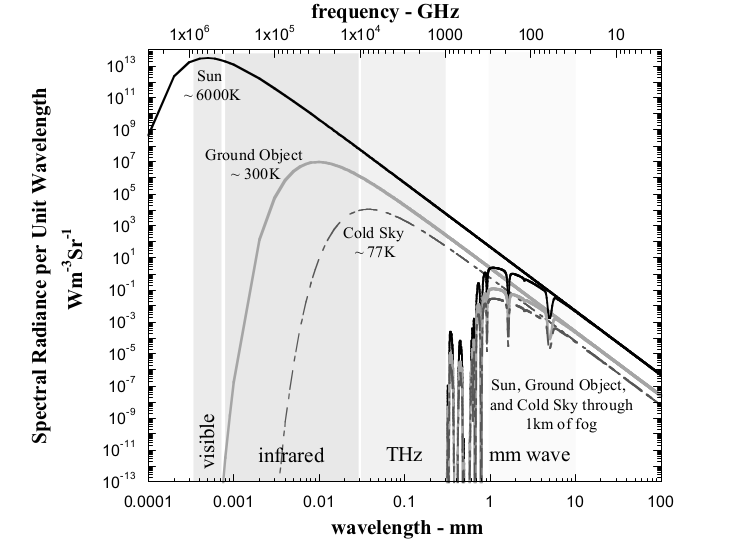
\includegraphics[width=0.8\textwidth]{imgs/attenuation}
	\caption{Loss bands within millimeter wave region allow for sensing in
	adverse weather conditions \cite{patel2016computational}.}
	\label{fig:attentuation}
\end{figure}

In recent years, the computer vision community has made dramatic progress on classification,
detection, tracking, and other problems with the development of deep neural
networks, using large labeled training datasets. However, vision alone cannot
solve certain problems such as position and velocity measurements with
satisfactory results, but radar systems excel at these. Additionally, the
presence of environmental conditions, such as rain, fog, smoke, and dust
significantly hinder visible system performances, but radar performance is
relatively unaffected in these situations \cite{patel2016computational}. Figure \ref{fig:attentuation} shows the atmospheric
attenuation of naturally emitted black-body radiation through 1 km of fog. 

In this thesis, we will cover the mathematics for determing range, velocity, and
estimating angle of arrival for targets in front of a FMCW radar. 
	% for INTRODUCTION in "intro.tex"
\chapter{Estimating Range}
As the name Frequency Modulated Continuous Wave (FMCW) implies, a FMCW radar is
a continuous time system which transmits and receives a periodic signal whose 
frequency has been modulated. As a periodic signal, the transmitted signal has
the complex form (with unit-normalized amplitude)
\begin{equation}
	\label{eq:complex-sinusoid}
	p(t) = e^{j2\pi f(t)t}.
\end{equation}
The typical frequency modulation used in FMCW radar systems is the sawtooth
modulation, given by
\cite{iovescufundamentals, wang2008digital}
\begin{equation}
	\label{eq:sawtooth}
	f(t) = f_c + \alpha (t - kT_c), \quad\text{for } kT_c \leq t < (k+1)T_c, \quad
	k \in \mathbb{Z}
\end{equation}
where $\alpha > 0$ is the chirp-rate  $\frac{df}{dt}$, $f_c$ is the base
carrier frequency (e.g. 77 GHz), and $T_c$ is the period of the chirp. To
simplify the calculations, we will deal with a single chirp until for range
calculations, thus the frequency for a single chirp is 
\begin{equation}
	f(t) = f_c + \alpha t \quad\text{for } 0\leq t < T_c.
\end{equation}

The maximum frequency of each chirp is 
\begin{equation}
	f_{max} \triangleq f_c + \alpha T_c,
\end{equation}
and the bandwidth $B$ of the signal is
\begin{equation}
	B = f_{max} - f_c = \alpha T_c.
\end{equation}

Combining the sawtooth frequency modulation (\ref{eq:sawtooth}) with the complex
sinusoid (\ref{eq:complex-sinusoid}), we get
the transmitted (TX) signal as
\begin{equation}
	p(t) = e^{j(2\pi f_c t+ \pi \alpha t^2)}.
\end{equation}

\begin{figure}[h]
	\centering
	\begin{subfigure}[b]{0.8\textwidth}
		\begin{tikzpicture}
			\begin{axis}[
			axis x line = bottom,
			axis y line = left,
			xlabel = $t$,
			ylabel=$f(t)$,
			xmin=0, xmax=8,
			ymin=0, ymax=3.2,
			xtick=\empty,
			ytick=\empty,
			xlabel near ticks,
			ylabel near ticks,
			extra x ticks={4,8},
			extra x tick labels={$T_c$, $2T_c$},
			extra y ticks={0, 1, 3},
			extra y tick labels={$0$, $f_c$, $f_{max}$},
			]
			\draw 
				(axis cs:1.5, 1.75)
				-| (axis cs:2, 2)
				node [near end, right]
				{$\alpha$};
			\addplot [
			domain=0:8,
			samples=100,
			color=black,
			]
			{(1 + 0.5*x)*(x<4)+(1+0.5*(x-4))*(x>4)};
			\end{axis}
		\end{tikzpicture}
		\label{fig:sawtooth}
		\caption{Example of sawtooth frequency modulation}
	\end{subfigure}
	\begin{subfigure}[b]{0.8\textwidth}
		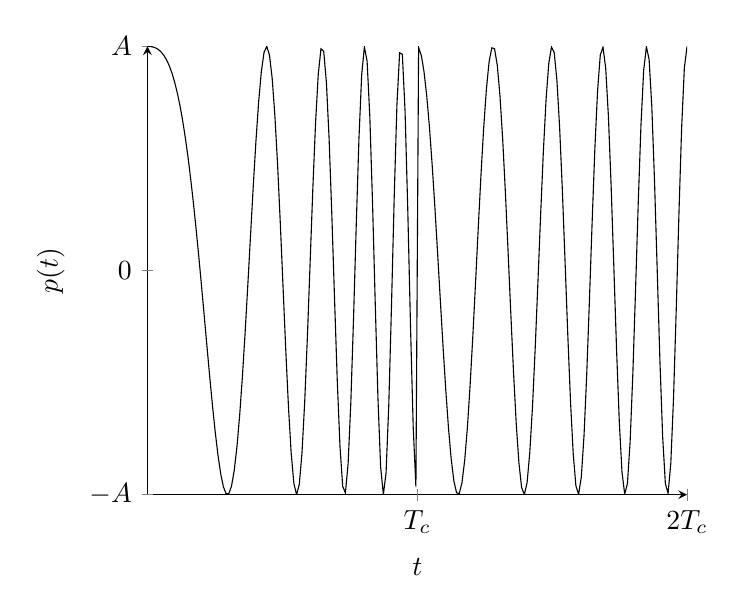
\begin{tikzpicture}
			\begin{axis}[
			axis x line = bottom,
			axis y line = left,
			xlabel = $t$,
			ylabel=$p(t)$,
			xmin=0, xmax=8,
			ymin=-1, ymax=1,
			xtick=\empty,
			ytick=\empty,
			xlabel near ticks,
			ylabel near ticks,
			extra x ticks={4,8},
			extra x tick labels={$T_c$, $2T_c$},
			extra y ticks={-1, 0, 1},
			extra y tick labels={$-A$, $0$, $A$},
			]
			\addplot [
			domain=0:8,
			samples=200,
			color=black,
			]
			{cos(deg(2*pi*((0.125 + 0.25*x)*(x<4)+(0.25+0.125*(x-4))*(x>4))*x)};
			\end{axis}
		\end{tikzpicture}
		\label{fig:pulse}
		\caption{Example of TX signal $p(t)$}
	\end{subfigure}
\end{figure}

Consider a target at a distance $d$ from the radar, such that the transmitted
(RX) signal reflects off the target and returns to the radar. This received signal
will be a time delayed version of the TX signal, where the time delay $\tau$ is
given by
\begin{equation}
	\tau = \frac{2d}{c}
\end{equation}
where $c$ is the speed of light. The RX signal thus has the form
\begin{equation}
	p(t-\tau)=e^{j(2\pi f_c (t-\tau) + \pi\alpha (t-\tau)^2)}.
\end{equation}

\begin{figure}[h]
	\centering
	\begin{tikzpicture}
		\begin{axis}[
		axis x line = bottom,
		axis y line = left,
		xlabel = $t$,
		ylabel=$f(t)$,
		xmin=0, xmax=8,
		ymin=0, ymax=3.2,
		xtick=\empty,
		ytick=\empty,
		xlabel near ticks,
		ylabel near ticks,
		extra x ticks={1,4,8},
		extra x tick labels={$\tau$,$T_c$, $2T_c$},
		extra y ticks={0, 1, 1.5, 3},
		extra y tick labels={$0$, $f_c$, $f_b$, $f_{max}$},
		]
		\draw[dashed] (axis cs:0, 1.5) -| (axis cs:1, 0);
			
		\addplot [
		domain=0:8,
		samples=100,
		color=black,
		]
		{(1 + 0.5*x)*(x<4)+(1+0.5*(x-4))*(x>4)};
		\addplot [
		domain=0:8,
		samples=100,
		color=red,
		]
		{(x<1)*1 + (1+0.5*(x-1))*(x>1)*(x<5) + (1+0.5*(x-5))*(x>5)};
		\end{axis}
	\end{tikzpicture}
	\label{fig:received}
	\caption{Frequency of RX signal (delayed by time $\tau$)}
\end{figure}

To recover $\tau$, and subsequently $d$, we define a new dechirped signal $r(t)$
as the product of the transmitted signal with the complex conjugate of the
received signal
\begin{align}
	r(t) &\triangleq p(t)p^*(t-\tau) \\
	&= e^{j(2\pi f_c t + \pi \alpha t^2)}e^{-j[2\pi f_c (t-\tau) + \pi\alpha (t-\tau)^2 ]} \\
	&= e^{j(2\pi f_c \tau - \pi \alpha \tau^2)}e^{j2\pi\alpha\tau t}.\label{eq:range}
\end{align}
Note, the first exponential in (\ref{eq:range}) only depends on $\tau$, so it is
a constant phase term. However, the second term varies according to a constant
frequency (named the beat frequency) $f_b$
\begin{equation}
	f_b \triangleq \alpha \tau.
\end{equation}
Recovering $f_b$ allows us to recover the distance $d$ as
\begin{equation}
	\label{eq:distance}
	d = \frac{c f_b}{2\alpha}
\end{equation}
The maximum beat frequency occurs when $\tau = T_c$, as any $\tau \in (T_c, 2T_c]$ will
appear as $\tau^*$
\begin{equation}
	\tau^* = \tau - T_c, \quad \tau \in (T_c, 2T_c]
\end{equation}
and thus the recovered distance $d^*$ will be less than the true range the
target is from the radar. From this, we can get our maximum recoverable distance
for a given chirp period
\begin{equation}
	d_{max} = \frac{c T_c}{2}.
\end{equation}
To recover the beat frequency $f_b$ from the dechirped signal, $r(t)$, we can
simply use the Fourier Transform to get
\begin{align}
	R_r(f) &= \int_{-\infty}^{\infty} r(t) e^{-j2 \pi ft} dt \label{eq:range-ft}\\
	&= \int_{-\infty}^{\infty} e^{j(2\pi f_c \tau - \pi \alpha \tau^2)}e^{j2\pi\alpha\tau t} e^{-j2\pi ft}dt\\
	&= e^{j(2\pi f_c \tau - \pi \alpha
	\tau^2)}\int_{-\infty}^{\infty}e^{-j2\pi(f - \alpha\tau ) t} dt\\
	&= e^{j(2\pi f_c \tau - \pi \alpha \tau^2)}\delta (f - \alpha \tau),
\end{align}
where $\delta(f)$ is the Dirac Delta function.

Now consider the case of multiple ($N$) objects at different distances $d_i$ from the radar.
\begin{equation}
	d_i \not = d_j \quad \text{for } i \not = j, \quad i,j \in [1, N]
\end{equation}
Each of these objects will reflect the transmitted chirp with a unique delay
$\tau_i$, and therefore will have a unique beat frequency corresponding to these
delays. Using the continuous time Fourier Transform, we can always resolve the
unique beat frequencies corresponding to the time delays. 

\begin{figure}[h]
	\centering
	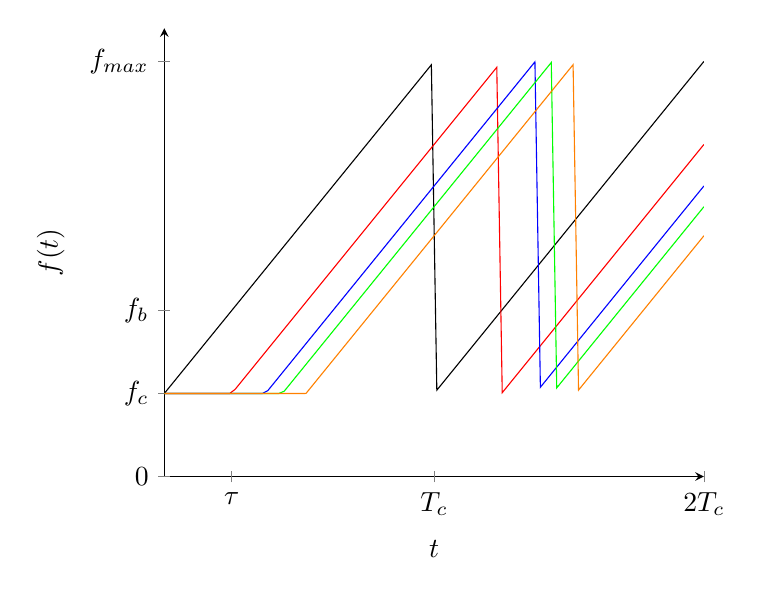
\begin{tikzpicture}
		\begin{axis}[
		axis x line = bottom,
		axis y line = left,
		xlabel = $t$,
		ylabel=$f(t)$,
		xmin=0, xmax=8,
		ymin=0.5, ymax=3.2,
		xtick=\empty,
		ytick=\empty,
		xlabel near ticks,
		ylabel near ticks,
		extra x ticks={1,4,8},
		extra x tick labels={$\tau$,$T_c$, $2T_c$},
		extra y ticks={0.5, 1, 1.5, 3},
		extra y tick labels={$0$, $f_c$, $f_b$, $f_{max}$},
		]
		\addplot [
		domain=0:8,
		samples=100,
		color=black,
		]
		{(1 + 0.5*x)*(x<4)+(1+0.5*(x-4))*(x>4)};
		\addplot [
		domain=0:8,
		samples=100,
		color=red,
		]
		{(x<1)*1 + (1+0.5*(x-1))*(x>1)*(x<5) + (1+0.5*(x-5))*(x>5)};
		\addplot [
		domain=0:8,
		samples=100,
		color=blue,
		]
		{(x<1.5)*1 + (1+0.5*(x-1.5))*(x>1.5)*(x<5.5) +
			(1+0.5*(x-5.5))*(x>5.5)};
		\addplot [
		domain=0:8,
		samples=100,
		color=green,
		]
		{(x<1.75)*1 + (1+0.5*(x-1.75))*(x>1.75)*(x<5.75) +
			(1+0.5*(x-5.75))*(x>5.75)};
		\addplot [
		domain=0:8,
		samples=100,
		color=orange,
		]
		{(x<2.1)*1 + (1+0.5*(x-2.1))*(x>2.1)*(x<6.1) +
			(1+0.5*(x-6.1))*(x>6.1)};
		\end{axis}
	\end{tikzpicture}
	\label{fig:received}
	\caption{Frequencies of reflected signals from multiple objects}
\end{figure}

However, in practice we must sample the received signal $r(t)$ with an
Analog-to-Digital converter (ADC), with sampling frequency $f_s = 1/T_s$. To retrieve
the beat frequencies, we take the $M$-point Discrete Fourier Transform (DFT) of
$r(t)$ for each chirp period
\begin{align}
	R_r[f] &= \sum_{m=0}^{M-1} r[mT_s] e^{-j\frac{2\pi}{M}fm} \label{eq:range-fft}\\
	&= \sum_{m=0}^{M-1} e^{j(2\pi f_c\tau -
	\pi\alpha\tau^2)}e^{j2\pi\alpha\tau mT_s} e^{-j\frac{2\pi}{M}fm}.
\end{align}
From this, we can see $R_r[f]$ has a peak when $f=MT_s\alpha\tau$, and since
$M$, $T_s$, and $\alpha$ are configured parameters, we can recover $\tau$ and
subsequently the distance $d$.
This processing can be done efficiently on hardware with the Fast Fourier Transform (FFT),
so this step is often called the Range-FFT. 

Since we are using the DFT, we can only resolve frequency components
separated by $1/T_c$, as $T_c$ is the observation window,
\begin{equation}
	\Delta f > \frac{1}{T_c}.	
\end{equation}
From (\ref{eq:distance}), we get the range-cell resolution
\begin{align}
	\Delta d &= \frac{c\Delta f}{2\alpha}\\
	\implies \Delta d &> \frac{c}{2\alpha T_c} = \frac{2}{2B}. \label{eq:range-res}
\end{align}


\chapter{Estimating Velocities}
To determine the velocity of an object, we can compare the phases of two chirps
reflected from the moving object. Recall from (\ref{eq:range}) that the first
exponential term in $r(t)$ has no dependence on $t$, so it fully describes the phase. We
can approximate this phase as a linear function of the time delay $\tau$, 
\begin{align}
	\phi(r(t)) &= 2\pi f_c \tau - \pi \alpha \tau^2 + 2\pi\alpha\tau t \\
	\implies \angle r(t) &\approx 2\pi f_c \tau.
\end{align}
For an object moving with velocity $v$ and initial range $d_0$, the time delay
$\tau$ is given by 
\begin{equation}
	\tau = \frac{2(d_0 + vt)}{c}, \label{eq:moving-tau}
\end{equation}
so the linear phase approximation becomes
\begin{equation}
	\phi(r(t)) \approx \frac{4\pi(d_0 + vt)}{\lambda},
\end{equation}
where $\lambda = \frac{c}{f_c}$ the wavelength of
the carrier signal. Now, the phase difference $\Delta \phi$ between two
dechirped signals separated by
$T_c$ is
\begin{equation}
	\Delta\phi = \frac{4\pi \Delta d}{\lambda},
\end{equation}
where $\Delta d$ is the distance the object travels over $T_c$ between the two
chirps. For an object traveling at a velocity $v$, this distance is
\begin{equation}
	\Delta d = v T_c, 
\end{equation}
so the phase difference becomes
\begin{equation}
	\label{phase_diff}
	\Delta\phi = \frac{4\pi v T_c}{\lambda}.
\end{equation}
However, phase difference is inherently ambiguous unless $|\Delta\phi|<\pi$, so
we find the maximum velocity measurable by two chirps spaced $T_c$ apart is
given by
\begin{equation}
	v_{max} = \frac{\lambda}{4 T_c}.
\end{equation} 

This two-chirp approach fails if we have multiple objects moving with different
velocities, but the same range at the time of measurement. The reflected chirps
will produce idential beat frequencies in this scenario, so the range processing
Fourier Transform will result in a single peak representing the combined signals
from the equidistant objects. In this case, we can use $K$ equally spaced chirps 
transmitted by the radar over a chirp frame $T_f = KT_c$. 

\begin{figure}[h]
	\centering
	\begin{tikzpicture}
		\begin{axis}[
		axis x line = bottom,
		axis y line = left,
		xlabel = $t$,
		ylabel=$f(t)$,
		xmin=0, xmax=8.5,
		ymin=0.5, ymax=5.2,
		xtick=\empty,
		ytick=\empty,
		xlabel near ticks,
		ylabel near ticks,
		extra x ticks={2,4,8},
		extra x tick labels={$T_c$, $2T_c$, $T_f =
			KT_c$},
		extra y ticks={0.5, 1, 5},
		extra y tick labels={$0$, $f_c$, $f_{max}$},
		]
		\addplot [
		domain=0:8,
		samples=100,
		color=black,
		]
		{(1 + 2*x)*(x<2) + (1+2*(x-2))*(x>2)*(x<4) + (1+2*(x-4))*(x>4)*(x<6) + (1+2*(x-6))*(x>6)*(x<8)};
		\end{axis}
	\end{tikzpicture}
	\label{fig:chirp-frame}
	\caption{Chirp frame $T_f$ consisting of $K$ chirps}
\end{figure}

Now we will need to use the full sawtooth frequency modulation as described in
(\ref{eq:sawtooth}), so $p(t)$ is
\begin{equation}
	p(t) = e^{j(2\pi f_c t+ \pi \alpha t^2 - 2\pi\alpha kT_c t)}.
\end{equation}
Then, the dechirped signal $r(t)$ will be
\begin{equation}
	r(t) = e^{j(2\pi f_c \tau - \pi \alpha \tau^2 + 2\pi\alpha\tau (t-kT_c))}.
\end{equation}
Again, we approximate by eliminating the quadratic components to get
\begin{equation}
	\phi (r(t)) \approx 2\pi (f_c + \alpha t_k)\tau,
	\label{eq:phase-approx}
\end{equation}
where 
\begin{equation}
	t_k \triangleq t - kT_c \quad \text{for }k\in\mathbb{Z}.
\end{equation}
Substituting (\ref{eq:moving-tau}) into (\ref{eq:phase-approx}) gives
\begin{align}
	\phi (r(t)) &\approx \frac{4\pi}{c}(f_c d_0 + f_c vt + \alpha d_0 t_k)\\
	&= 2\pi (f_c \tau_0 + f_d t + t_k f_{\tau})\\
	&= 2\pi (f_c \tau_0 + f_d k T_c + (f_{\tau} + f_d) t_k)
\end{align}
where $\tau_0$ is the initial time delay, $f_d$ is the Doppler Frequency, and
$f_{\tau}$ is the range-beat-frequency, as defined below.
\begin{align}
	\tau_0 &\triangleq \frac{2d_0}{c}\\
	f_d &\triangleq \frac{2v}{c} f_c\\
	f_{\tau} &\triangleq \alpha\tau_0
\end{align}
For each $k$-th chirp, we compute $R_r(f,k)$ as in (\ref{eq:range-ft}), which
contains the range information for the objects,
\begin{align}
	R_r(f,k) &= \int_{\tau}^{T_c} r(t_k)e^{-j2\pi f t_k}dt_k\\
	&= \int_{\tau}^{T_c} e^{j\phi(r(t_k))}e^{-j2\pi f t_k}dt_k\\
	&= \int_{\tau}^{T_c} e^{j2\pi (f_c \tau_0 + f_d k T_c + (f_{\tau} + f_d) t_k)}e^{-j2\pi f t_k}dt_k.
\end{align}
The absolute value $|R_r(f,k)|$ is obtained for $f = f_d + f_\tau$, and, in
general, $f_\tau >> f_d$, so we can resolve the ranges as before.
Now, since the term $f_dkT_c$ depends on $k$, we see $R_r(f,k)$ is a 
function of $k$, with sampling period $T_c$, observed $K$ consecutive times over the course of the chirp frame
$T_f$. Each of these $k$ spectrums will have a different phase which combines the
phase contributions from each object at the corresponding range with different
velocities. This spectrum is described by the following Discrete Fourier Transform
\begin{equation}
	\label{eq:velocity-fft}
	R(f, n) = \sum_{k=0}^{K-1}R_r(f, k) e^{-j\frac{2\pi}{K}kn},
\end{equation}
which achieves maximum absolute value (i.e. a peak) when 
\begin{equation}
	n = f_d T_c.
\end{equation}

In the case of multiple objects at the same range, but with different
velocities, we will have peaks corresponding to the Doppler Frequencies of each
object, enabling us to resolve the different velocities. Since we are using the
DFT, we can derive the velocity resolution as we did the range resolution in
(\ref{eq:range-res}), where the observation window here is the frame time $T_f$,
\begin{equation}
	\Delta v = \frac{c}{2 K T_c f_c} = \frac{c}{2 f_c T_f}.
\end{equation}

This spectrum is computed using the Fast Fourier Transform method, so we call
this step the Doppler-FFT. By reordering the samples of $r(t)$ into a 2D matrix
$\bm{R}$ where each row is the samples from one chirp period $T_c$ with $K$ rows
(i.e. $K$ chirps), we can compute the Range-FFT and Doppler-FFT as a 2D FFT over
the data matrix $\bm{R}$. 

\chapter{Computing Angle of Arrival}
If the radar has at least 2 transmit-receive antenna pairs, we can use the
phase change in the Fourier Transforms that arises from the slight difference
in range the object has to each receiving antenna to calculate the angle of
arrival (AoA) for the received signal. 

% drawing of antenna and \delta d
\begin{figure}[h]
	\center
	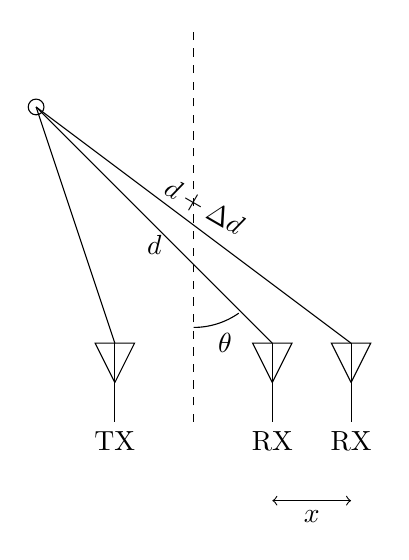
\begin{tikzpicture}
		\draw (1,0.5) -- (0.75, 1) -- (1.25, 1) -- (1,0.5);
		\draw (1, 1) -- (1,0) node[below] {RX};
		\draw (2,0.5) -- (1.75, 1) -- (2.25, 1) -- (2,0.5);
		\draw (2, 1) -- (2,0) node[below] {RX};
		\draw[<->] (1,-1) to node[below] {$x$} (2, -1);
		\draw (-1,0.5) -- (-0.75, 1) -- (-1.25, 1) -- (-1,0.5);
		\draw (-1, 1) -- (-1,0) node[below] {TX};
		\draw (-2,4) circle [radius=0.1];
		\draw (-2,4) to node[below] {$d$} (1,1);
		\draw (-2,4) to node[above, rotate=330] {$d+\Delta d$}  (2,1);
		\draw (-2,4) to (-1,1);
		\draw[dashed] (0,0) to (0,5);
		\draw (0,1.2) arc (-90:-55:1);
		\draw (0.4, 1) node {$\theta$};
	\end{tikzpicture}
	\caption{Angle of Arrival Problem}
	\label{fig:angle-of-arrival}
\end{figure}

\section{Geometric Estimation}
From Figure \ref{fig:angle-of-arrival}, we can derive the phase difference
between the received signals $r_1(t)$ and $r_2(t)$ at two different antennas
separated by a distance $x$. Let $d$ be the distance the received signal
$r_1(t)$ travels to reach the first antenna and $d + \Delta d$ be the distance
the reflected signal $r_2(t)$ travels to reach the second antenna
\cite{iovescu2017fundamentals}. Assuming the
radar signal is a planar wavefront, the geometry shown in Figure
\ref{fig:geometric-aoa} gives
\begin{equation}
	\Delta d = x \sin \theta. 
\end{equation}
\begin{figure}
	\center
	\begin{tikzpicture}
		\draw[dashed] (0,-0.5) to (0,6);
		\draw (2,0) to node[below] {$x$} (4,0);
		\draw (4,0) to node[above, rotate=315] {$\Delta d$} (3, 1);
		\draw (2,0) to (3, 1);
		\draw (2.8, 0.8) -- (3, 0.6) -- (3.2, 0.8);
		\draw (2.4, 0) arc (0:45:0.4) node[right] {$\theta$};
		\draw (2,0) to (-1, 3.3);
		\draw (4,0) to (-1,5);
		\draw (0,1.8) arc (-90:-45:0.4) node[below] {$\theta$};
		\draw (2,0) to (2,-0.5);
		\draw (4,0) to (4, -0.5);
	\end{tikzpicture}
	\caption{Geometric Approach for Estimating Angle of Arrival}
	\label{fig:geometric-aoa}
\end{figure}

Now, the phase difference $\Delta \phi$ is given by
\begin{equation}
	\Delta \phi = \frac{2\pi \Delta d}{\lambda}.
\end{equation}
Now, we can compute the angle of arrival $\theta$ as 
\begin{equation}
	\theta = \sin^{-1}(\frac{\lambda\Delta\phi}{2\pi x}).
\end{equation}
However, since $\Delta\phi$ depends on $\sin\theta$, our accuracy degrades for
large $\theta$, as $\sin\theta \approx \theta$ only for small $\theta$. 

As before, the phase difference $|\Delta\phi |<\pi$ to be unambiguous, so we
find
\begin{equation}
	\frac{2\pi x}{\lambda} \sin\theta < \pi,
\end{equation}
and the maximum field of view for two TX-RX antenna pairs spaced $x$ apart is 
\begin{equation}
	\theta_{max} = \sin^{-1}(\frac{\lambda}{2x}).
\end{equation}
Clearly, the largest angular field of view for two antenna pairs with this
approach occurs when the antenna spacing is
\begin{equation}
	x = \frac{\lambda}{2},
\end{equation}
giving $\theta_{max} = \pm\frac{\pi}{2}$.

\section{Multiple Signal Classification (MUSIC)}
For Multiple Input Multiple Output (MIMO) FMCW radar systems, we can use more
sophisticated angle of arrival techniques based on subspaces. Let
us assume we have an arbitrary array of $L$ virtual transmit-receive antenna pairs, with an
array response vector $\bm{a}(\theta)$. This response vector maps the direction
of arrival $\theta$ to the signal phase shift at each of the $L$ virtual antenna
pairs. For a set of $N$ objects, we will have $N$ return signals $r(t)$
returning to the antenna array. Let $\bm{x}(t)$ be the superposition of the
signals so that \cite{bresler2017hilbert}
\begin{align}
	\bm{x}(t) &= \sum_{n=1}^N s_n(t) \bm{a}(\theta_n)\\
	&= \bm{A}(\bm{\theta})\bm{s}(t)
\end{align}
where
\begin{align}
	\bm{A}(\bm{\theta}) &= [\bm{a}(\theta_1), \bm{a}(\theta_2), \dots, \bm{a}(\theta_N)]\\
	\bm{\theta} &= [\theta_1, \theta_2, \dots, \theta_N]^T\\
	\bm{s}(t) &= [s_1(t), s_2(t), \dots, s_N(t)]^T.
\end{align}
If we sample $\bm{x}(t)$ at $M$ timesteps, we get the following matrix equation
\begin{equation}
	\bm{X} = \bm{A}(\bm{\theta})\bm{S}
\end{equation}
where $\bm{X}$ is a $L \times M$ matrix of samples, $\bm{A}(\bm{\theta})$ is a
$L\times N$ matrix function, and $\bm{S}$ is a $N\times M$ matrix
\begin{align}
	\bm{X} &= [\bm{x}(t_1), \bm{x}(t_2), \dots, \bm{x}(t_M)]\\
	\bm{S} &= [\bm{s}(t_1), \bm{s}(t_2), \dots, \bm{s}(t_M)].
\end{align}
Since $\bm{X}$ is the product of a $L\times N$ matrix and a $N\times M$ matrix,
we have that $rank(\bm{X}) = N$, assuming $\bm{A}(\bm{\theta})$ has full column
rank and $\bm{S}$ has full row rank. This corresponds to the number of objects
whose angular position we are trying to compute. Now, since the range space of
$\bm{X}$, $\mathcal{R}(\bm{X})$, is the same subspace as the range space of
$\bm{A}(\bm{\theta})$
\begin{equation}
	\mathcal{R}(\bm{X}) = \mathcal{R}(\bm{A}(\bm{\theta})),
\end{equation}
we can use the Singular Value Decomposition (SVD) of $\bm{X}$ to recover
$\theta_i$. The SVD of $\bm{X}$ is given by
\begin{align}
	\bm{X} &= \bm{U} \bm{\Sigma} \bm{V}^H\\
	&= [\bm{U_s} | \bm{U_n}] \begin{bmatrix} \Sigma_s & 0 \\
	0 & \bm{0} \end{bmatrix} \bm{V}^H
\end{align}
where the left singular vectors have been separated into those corresponding
with the nonzero singular values ($\bm{U}_s$) and those corresponding to the
zero singular values ($\bm{U}_n$). From linear algebra, we know the columns of
$\bm{U}_s$ span the signal subspace $\mathcal{R}(\bm{X})$ and the columns of
$\bm{U}_n$ span the left nullspace $\mathcal{N}{\bm{X}^H})$ of $\bm{X}$, which
is the orthogonal complement of the signal subspace \cite{meyer2000matrix}. In this context, we will
call this subspace the noise subspace
\begin{align}
	\text{span}(\bm{U_n}) &= \mathcal{N}(\bm{X}^H) \\
	&= \mathcal{R}(\bm{X})^\perp\\
	&= \mathcal{R}(\bm{A}(\bm{\theta}))^\perp.
\end{align}
Now, if we sweep $\theta \in [0, 2\pi)$, $\bm{a}(\theta)$ wil lie in the left
nullspace of $\bm{X}$ when $\theta=\theta_i$, where $\theta_i$ are the desired
angles of arrival we are estimating, 
\begin{equation}
	\theta = \theta_i \iff \bm{U}_n^H \bm{a}(\theta) = 0.
\end{equation}
The Multiple Signal Classification (MUSIC)
algorithm leverages this fact by finding the peaks in \cite{schmidt1986multiple}
\begin{equation}
	g(\theta) = \frac{1}{\|\bm{U}_n^H \bm{a}(\theta)\|^2}.
\end{equation}

%\section{ESPRIT}

\chapter{Conclusion}
In this work, the processing chain for linear frequency-modulated 
continuous-wave radars was explored. We demonstrated how the sawtooth frequency modulation
gives rise to the beat-frequency phenomenon from the combined transmit-receive
signals and contains the range information via the time delay. Furthermore, we
investigated the influence of an object's velocity on the phases for return
signals corresponding to different chirps and how to leverage this information
with a second Fourier transform to recover the Doppler frequencies. Next, we
discussed angular position estimation for multiple-input multiple-output radar
systems, first by a simple geometric estimation and second by the
subspace-based multiple signal classification (MUSIC) algorithm. Finally, we
presented simulated results of a 77 GHz FMCW radar system based on Texas Instruments's
IWR 1443 chip and investigated the effects of several configurable system
parameters on range and velocity detection performance.



%%%%%%%%%%%%%%%%%%%%%%%%%%%%%%%%%%%%%%%%%%%%%%%%%%%%%%%%%%%%%%%%%%%%%%%%%%%%%%%
% APPENDIX
%
\appendix
%\include{apx}

\backmatter

%%%%%%%%%%%%%%%%%%%%%%%%%%%%%%%%%%%%%%%%%%%%%%%%%%%%%%%%%%%%%%%%%%%%%%%%%%%%%%%
% BIBLIOGRAPHY
%
\bibliographystyle{IEEE_ECE}
% Put references in BibTeX format in thesisrefs.bib.
\bibliography{thesisrefs}


%%%%%%%%%%%%%%%%%%%%%%%%%%%%%%%%%%%%%%%%%%%%%%%%%%%%%%%%%%%%%%%%%%%%%%%%%%%%%%%
% AUTHOR'S BIOGRAPHY
% As of 10/03/2011, Author's Biography or Vita no longer accepted by Grad College

\end{document}
\endinput
